\chapter{Test}

\section{Analisi dei dati}
La predizione dei risultati \`e stata implementata sia nel software \textit{Android} sia sul computer. Nel codice eseguito su dispositivo mobile \`e stato adoperato solamente il KNN per via della facilita' d'implementazione e non \`e stato  utilizzato per testare la precisione, ma per verificare il corretto funzionamento dell'applicazione. Invece su computer, presi i dati serializzati dal software mobile, sono stati applicati tutti gli algoritmi di apprendimento elencati precedentemente e gia' tutti implementati da librerie di terze parti per verificare la precisione dei dati. Il linguaggio scelto su computer \`e \textit{Python} per via del suo buon supporto all' apprendimento automatico tramite la libreria \textit{sklearn}.



\section{Piano dei test}
Per testare l'effettivo funzionamento dell'applicazione ho usato alcune stanze di casa mia ed ho assegnato a ciascuna di esse una \textit{label}. Qui di seguito una piccola piantina rappresentante le stanze utilizzate:

\begin{figure}[H]
\centering
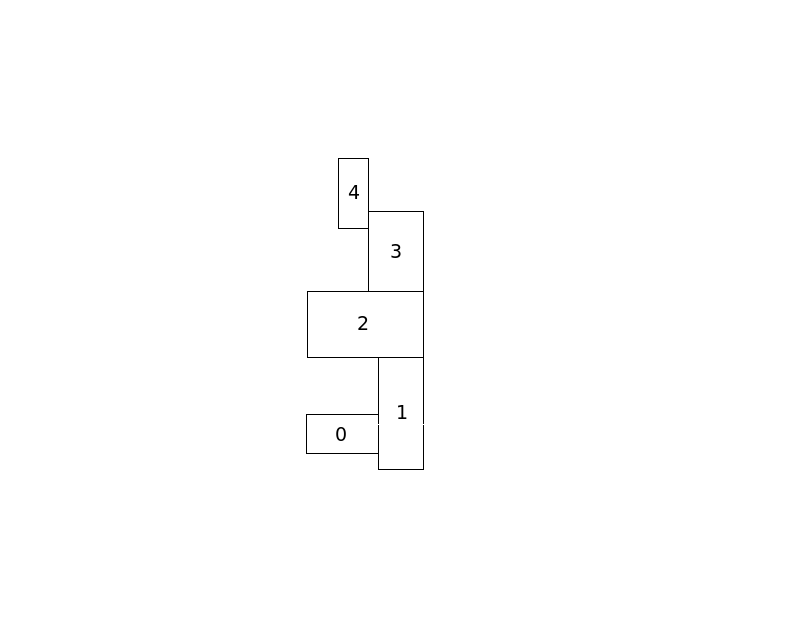
\includegraphics[width=0.7\linewidth]{img/test_pianta_casa}
\caption{Una piccola raffigurazione delle stanze usate per le prove con sopra scritto la \textit{label} assegnata}
\label{fig:test_pianta_casa}
\end{figure}

Sono stati raccolti circa 18000 campioni di onde magnetiche. La suddivisione fra addestramento e test \`e 70/30. La misura delle performance \`e l'errore sui test quindi  $1 - \dfrac{\# predizioni\, azzecate}{\# predizioni\,totali}$

\section{Caratteristiche dei dati}
Dai grafici qui di seguito possiamo notare che c'e' sovrapposizione fra i dati, quindi \`e presente del rumore nei dati.
\begin{figure}[H]
	\centering
	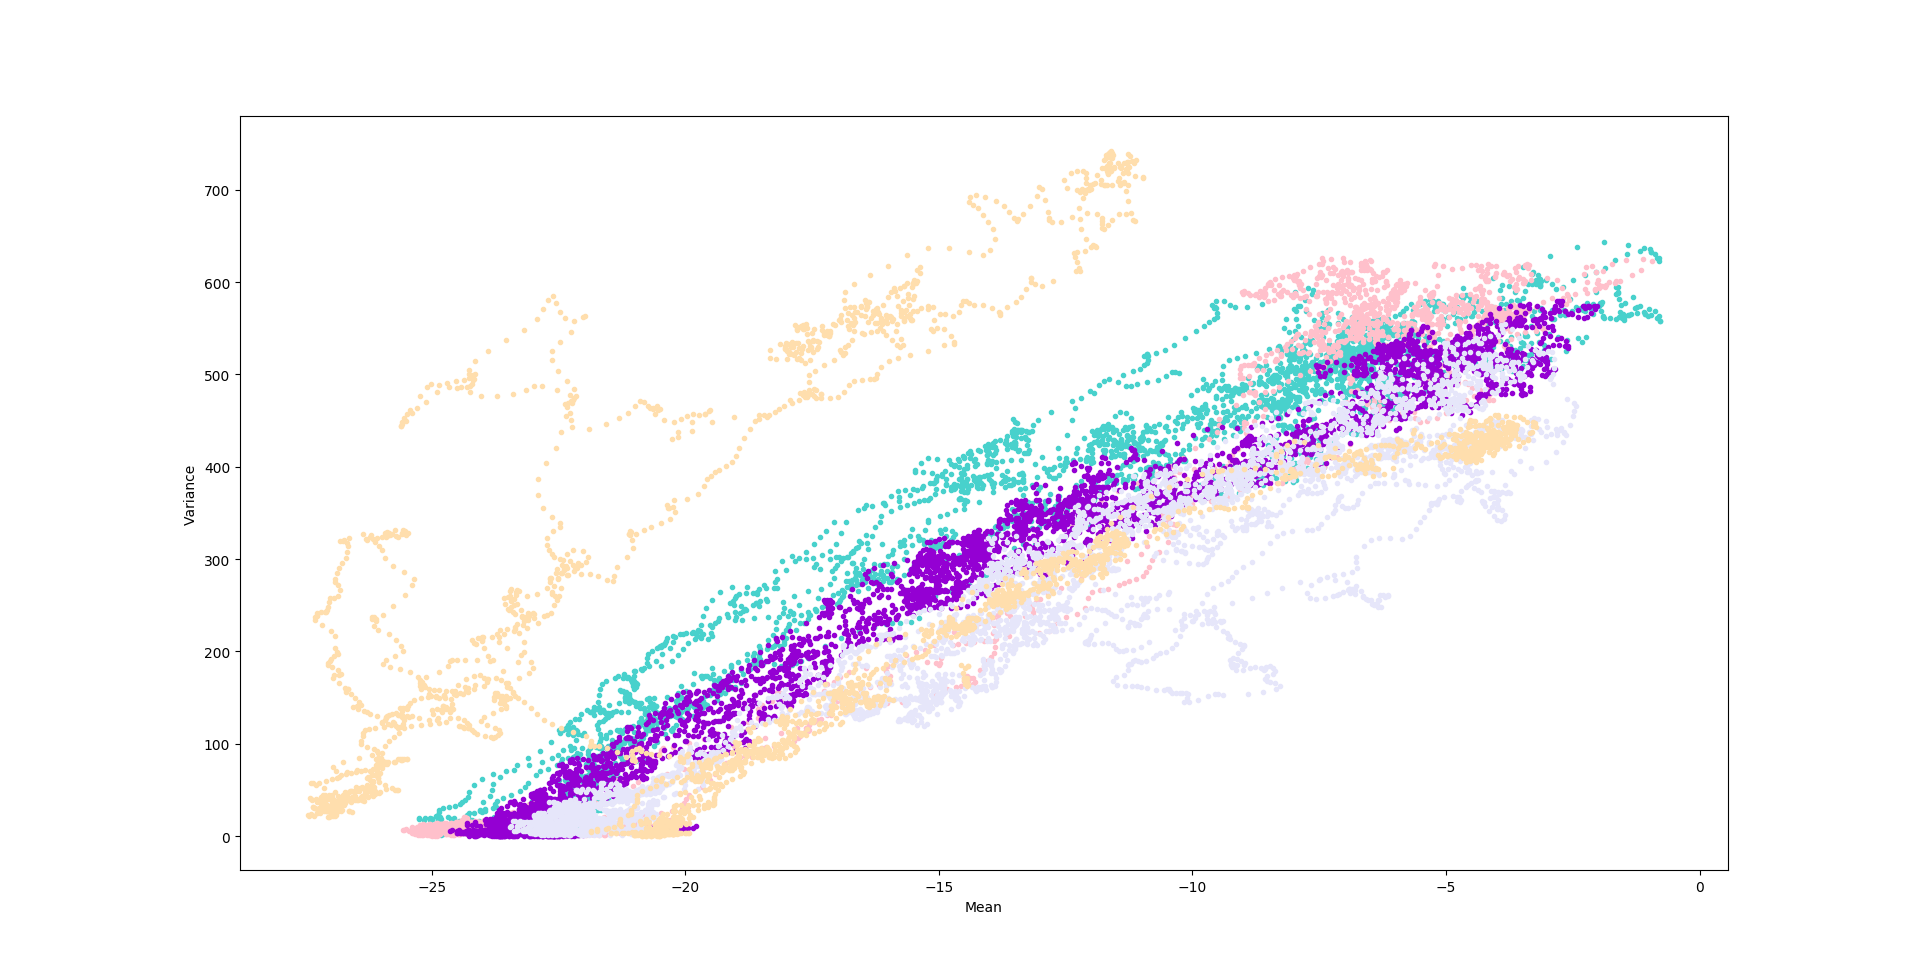
\includegraphics[width=1\linewidth]{img/plot_features}
	\caption{Grafico in 2 dimensioni della media e varianza di tutte le onde magnetiche. I colori dei punti rappresentano le etichette}
	\label{fig:plotfeatures}
\end{figure}

La causa del rumore sono i sensori che offrono una misurazione non precisa. Per risolvere, almeno in parte questo problema, \`e stato usato il \textit{filtro di Kalman} durante il preprocessamento dei dati per pulire il rumore sui dati.

\section{Codice per l'analisi dati col \textit{knn}}
\lstinputlisting[language=Python]{code/sklearn_classify.py}
Nel codice \`e stato preso come esempio il \textit{knn}, ma si puo' fare la stessa cosa con tutti gli altri classificatori. E' stata saltata la fase di pre-elaborazione dei dati perche' poco importante nel nostro caso studio mentre ci concentriamo di piu' sulla validazione degli iperparametri e la predizione di risultati per poi terminare con il calcolo dell'accuratezza. Da notare che la validazione \`e stata fatta tramite \textit{cross validation} tramite la tecnica della \textit{grid search}, che consiste semplicemente nel provare tutti i valori all'interno di \textit{$h\_params\_knn$} e selezionare quello con l'accuratezza migliore. Il paraemtro \textit{cv=5} significa che il dataset d'addestrameto \`e stato suddiviso in 5 parti. Dopo la validazione \`e stato preso il k migliore e sono stati confrontati i risultati fra un \textit{knn} con i migliori iperparametri e quelli di \textit{default}. I risultati di tale prova sono piu' avanti.


\section{Classificatori a confronto}
Qui di seguito vediamo i risultati ottenuti da ciascun classificatore con un istogramma:

\begin{figure}[H]
	\centering
	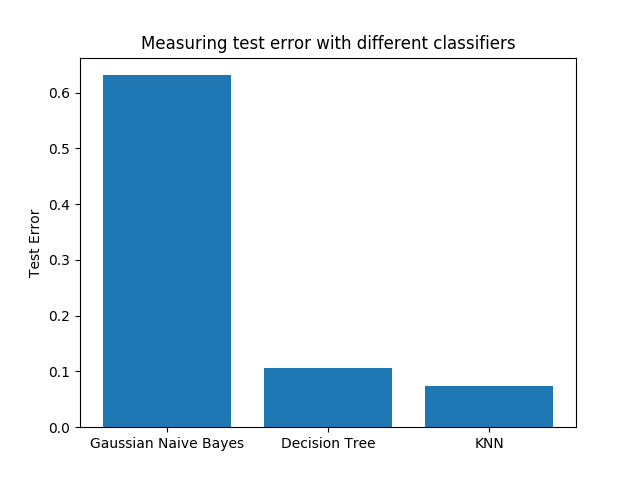
\includegraphics[width=0.7\linewidth]{img/test_errors}
	\caption{Percentuale d'errore nei test dei classificatori}
	\label{fig:testerrors}
\end{figure}

come possiamo notare \textit{Gaussian Naive Bayes} \`e totalmente inadatto alla classificazione di onde magnetiche mentre gli alberi di decisione e \textit{K Nearest Neightbours} si comportano molto bene, con risultati leggermente migliori in quest'ultimo.
A questo punto qualcuno potrebbe pero' pensare che gli ultimi 2 modelli si sono sovradattati agli esempi (\textit{overfitting}) ed avrebbe ragione, perche' applicando la \textit{cross validation} abbiamo risultati diversi da quelli precedenti.

\begin{figure}[H]
	\centering
	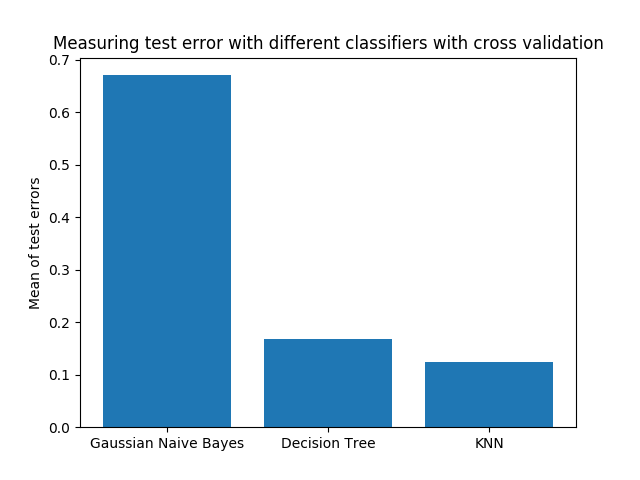
\includegraphics[width=1\linewidth]{img/test_errors_cross_validation}
	\caption{Percentuale d'errore nei test dei classificatori con la \textit{cross validation}}
	\label{fig:testerrorscrossvalidation}
\end{figure}

Adesso visualizziamo gli errori per etichetta:

\begin{figure}[H]
	\centering
	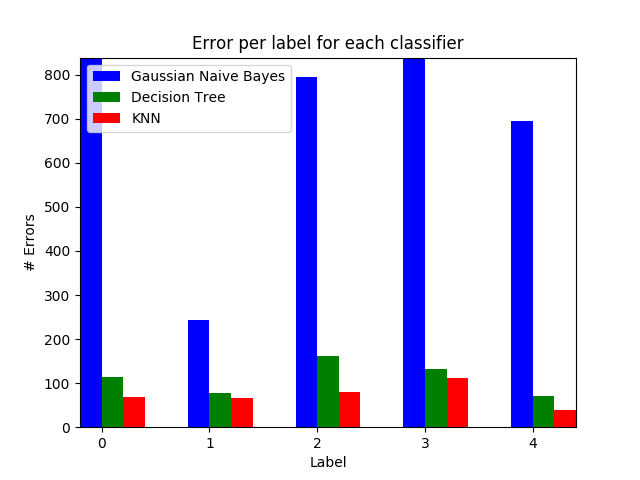
\includegraphics[width=0.7\linewidth]{img/test_error_per_label}
	\caption{Numero di errori nella predizione per etichetta}
	\label{fig:testerrorperlabel}
\end{figure}
\medskip
\begin{figure}[H]
	\centering
	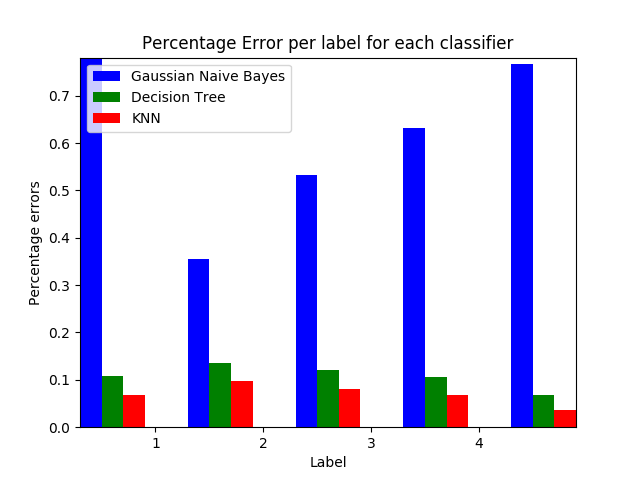
\includegraphics[width=0.7\linewidth]{img/percentage_test_errors_per_label}
	\caption{Percentuale di errore nella predizione per etichetta. Le barre blu rappresentano i risultati dei classificatori \textit{cross-validati} mentre i rossi sono quelli senza.}
	\label{fig:percentagetesterrorsperlabel}
\end{figure}

\section{Analisi del Knn al variare dell'iper parametro k}
Un grafico interessante da analizzare \`e l'accuratezza del \textit{Knn} al variare di K. L'accuratezza \`e intesa come la percentuale di predizioni azzeccate sull'insieme di test, inoltre i risultati sono stati \textit{cross validati}.
\begin{figure}[H]
	\centering
	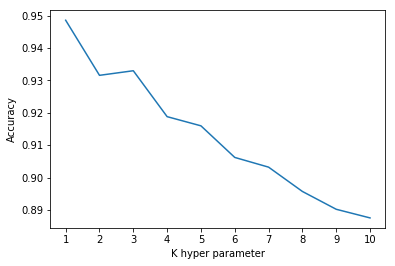
\includegraphics[width=0.7\linewidth]{img/accuracy_knn}
	\caption{Accuratezza del knn al variare di K}
	\label{fig:accuracyknn}
\end{figure}
In base a questo grafico potremmo supporre di prendere \textit{Knn} con k = 1 ma sarebbe un grave errore che porterebbe a pessimi risultati nel mondo reale. Come mai? Innanzitutto spieghiamo cio' che succede col 1-nn: per ogni nuovo punto la sua etichetta sara' quella del vicino piu' prossimo. I nostri problemi si possono ricondurre all'\textit{overfitting}, che riassumendo vuol dire che il nostro modello ha imparato troppo bene (a memoria) i nostri dati. Invece se impostiamo un k troppo alto avremo lo stesso risultato l'\textit{underfitting} ma per il motivo contrario, cioe' il nostro modello ha imparato troppo poco dai dati. Per notare veramente gli effetti dell'\textit{overfitting}, adesso vedremo su un piano cartesiano le sue conseguenze prendendo come esempio una classificazione binaria su due attributi dove ogni punto sara' colorato di blu e rosso in base alla sua etichetta. Nel grafico \`e stata tracciata una linea nera di separazione fra le due aree rosse e blu per indicare che i punti i quali andranno nell'area rossa saranno classificati come rossi dal knn e viceversa per i blu.

\begin{figure}[H]
	\centering
	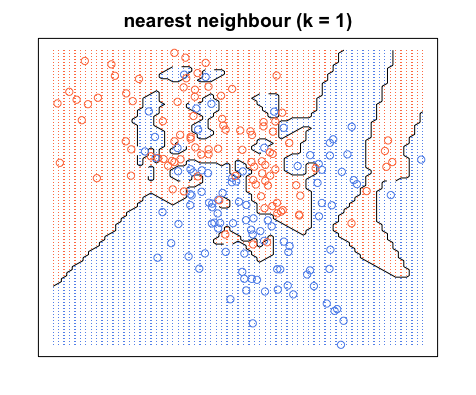
\includegraphics[width=0.7\linewidth]{img/1nearestneigh}
	\caption{Classificazione binaria con il 1-nn}
	\label{fig:1nearestneigh}
\end{figure}

\begin{figure}[H]
	\centering
	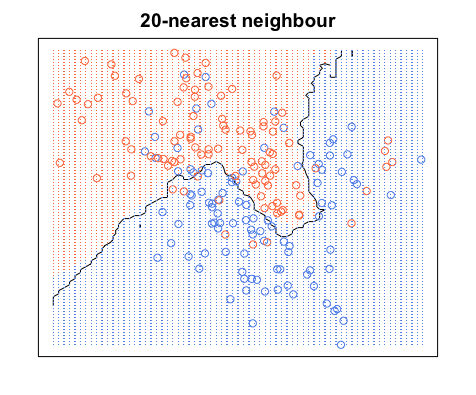
\includegraphics[width=0.7\linewidth]{img/20nearestneigh}
	\caption{Classificazione binaria con il 20-nn}
	\label{fig:20nearestneigh}
\end{figure}

Si puo' notare bene che con k=1 abbiamo sicuramente meno errori di classificazione nel nostro dataset, ma stiamo comunque ignorando il fatto che alcuni punti rossi fra i blu possono essere frutto di errore umano, sensori o di una qualsiasi fonte di dati e che quindi andrebbero ignorati. Questo risultato si ottiene andando a controllare l'etichetta di molti piu' vicini ed \`e cio' che avviene con k = 20.
Per evitare problemi di \textit{overfitting} ed \textit{underfitting} \`e necessario usare altre metriche per valutare l'efficacia del nostro modello.

\begin{figure}[H]
	\centering
	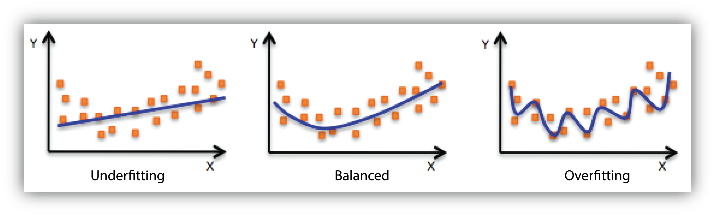
\includegraphics[width=1\linewidth]{img/underfittingoverfitting}
	\caption{\textit{Underfitting} ed \textit{overfitting} nella regressione}
	\label{fig:underfittingoverfitting}
\end{figure}

Una soluzione a questo problema \`e possibile ottenerla dalle curve di validazione che mostrano a grafico la complessita' del modello sull'asse x, quindi per esempio al variare di uno o piu' iperparamentri mentre sull'asse y l'errore sia sull'insieme di validazione che sull'insieme di addestramento.

\begin{figure}[H]
	\centering
	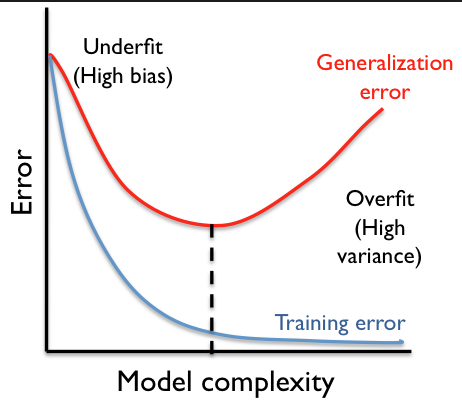
\includegraphics[width=0.7\linewidth]{img/validation_curve}
	\caption{Curve di validazione}
	\label{fig:validationcurve}
\end{figure}

Come si vede dal grafico, si dice che quando c'e' \textit{overfitting} si ha un altra varianza? Cosa vuol dire? Che stiamo modellando anche il rumore generato dai dati e cio' porta a cattive prestazioni quando ci arrivano nuove etichette da predire. Per \textit{High bias} si intente semplicemente un alto errore sulle predizioni delle etichette.
\section{Analisi del rumore durante la cattura dei dati}
Per analizzare la correttezza dei nostri dati l'approccio usato \`e stato quello di posizionarsi fermo in un punto e verificare tramite grafico che tutti i punti catturati dal magnetometro fossero concentrati in una piccola area del grafico. Purtroppo non \`e stato cosi' e ce lo dimostrano i grafici dove \`e stato messo nell'asse X il valore X catturato e sull'asse Y il valore Y.

\begin{figure}[H]
	\centering
	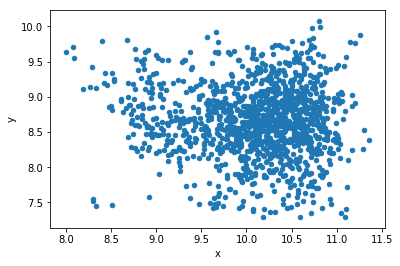
\includegraphics[width=0.7\linewidth]{img/xystand}
	\caption{Valori del magnetometro rispetto agli assi x ed y stando fermo}
	\label{fig:xystand}
\end{figure}



\section{Un rimedio ingenuo al rumore}
Un approccio ingenuo per risolvere il problema al rumore potrebbe essere quello di prendere meno dati per etichetta. Il seguente grafico pero' ci mostra che cio' non \`e vero

\begin{figure}[H]
	\centering
	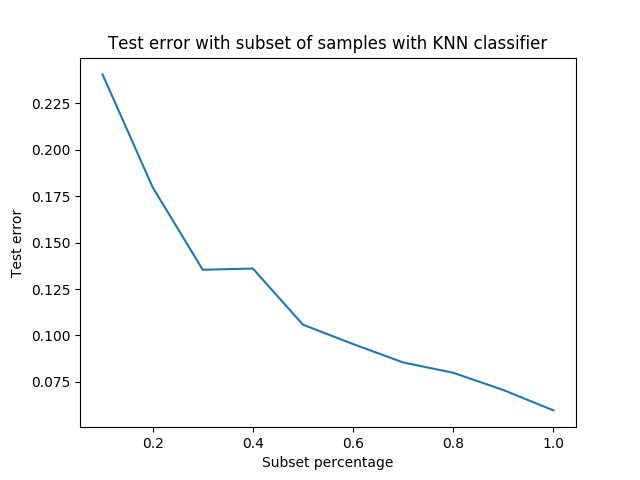
\includegraphics[width=0.7\linewidth]{img/rumor_graph_knn}
	\caption{Percentuale d'errore al variare della grandezza dell'insieme di addestramento con KNN}
	\label{fig:rumorgraphknn}
\end{figure}

Notiamo che questo grafico dimostra che all'aumentare del dataset otteniamo risultati piu' accurati poiche' ci stiamo avvicinando alla media e varianza della popolazione.

%Ricorda di far vedere falsi positivi e veri negativi nei test